

\noindent 
\textbf{\stepcounter{zadatak}
\thecjelina.\thezadatak.}
Na valjak polumjera $R$ i mase $M$ koji se može rotirati oko horizontalne osi namotana je nit na koju je obje\v{s}en uteg mase
$m$ (vidi skicu). Kolika će biti kutna brzina valjka u trenutku kad uteg padne s visine $h$?
\begin{figure}[h]%{r}{0.7\textwidth} % Inline image example
  \begin{center}
    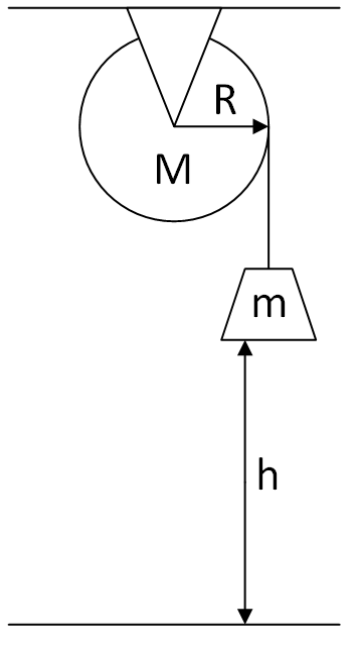
\includegraphics[scale=0.40]{../05_Kruto_tijelo/Zadatak_R901.png}
  \end{center}
  %\caption{Fish}
\end{figure}


